% Hadron-Hadron Scatteing
%%%%%-------PROVA-------------
%\documentclass[12pt]{report}
%\usepackage[british]{babel}
%\usepackage{amsmath}
%\usepackage{amsfonts}
%\usepackage{amssymb}
%\usepackage{geometry}
%\geometry{hmargin={2cm,2cm},vmargin={2cm,2cm}}
%\usepackage{caption}
%\captionsetup{format=hang}
%\usepackage{graphicx}
%\usepackage{enumitem}
%\usepackage{float}
%
%
%
%\usepackage[colorlinks=true, linkcolor=blue]{hyperref} %to use autoref
%%%%%-------------------------

%\begin{document}


\chapter{Hadron-Hadron Scattering}
\label{chap:Hadron-HadronScattering}

In a high energy proton-proton collision we can have either soft or hard processes.
Most of the time the hard processes are accompanied by soft interactions, occurring along the hadron interaction.
While the hard processes as the Higgs boson production, or the high $p_T$ jet production are well understood using perturbative QCD, the soft processes as the underlying event, the hadronization are not so well understood. In fact, these processes involving a low energy scale at which perturbative series expansion of QCD breaks down, are studied with non perturbative approaches. 

This chapter gives a theoretical introduction on some basic elements of perturbative QCD theory: the QCD factorization theorem, the fixed-order approach in perturbative QCD calculations for the partonic cross-section and the PDF.  
%and finally the all-orders approaches (e.g. the parton showers).

\noindent Then, it is described the parton shower with the  Initial and Final State Radiations. The effects of Multi Parton Interactions and other important processes in the simulation of High Energy Physics events in particular on the basic aspect of \textsc{pythia}8 generator.


\section{QCD factorization theorem}

The fundamental idea for the description of a hadron-hadron collision is that hadrons are made-up from partons that, at some high energy scale, can be seen as free. So the hadron-hadron interaction can be seen as an interaction between two free partons, given a sufficiently high energy scale for the interaction.
\\
This idea was developed in the framework of the deep inelastic scattering, and the Bjorken scaling observation confirms it \cite{Bjorken:1968dy}. The generalization of this concept leads to the \textit{QCD factorization theorem}. 
\\   
The factorization theorem was introduced first by Drell and Yan \cite{DRELL1971578}. 
The hadron-hadron scattering cross-section is described in terms of partons extending the formalism used for deep inelastic scattering, through the following factorized formula:
%\begin{equation}
%\sigma_{AB}=\displaystyle\int dx_a\,dx_b\,f_{a/A}(x_a)\,f_{b/B}(x_b)\,\hat{\sigma}_{ab \rightarrow X}\quad .
%\label{eq:factorization1}
%\end{equation}
%Where $X$ is a partonic/leptonic state and $a\,(b)$ a quark or an antiquark in the hadron $A\,(B)$. The $\sigma_{AB}$ is the hadronic cross-section while $\sigma_{ab\rightarrow X}$ is the partonic cross section that can be calculated using perturbative QCD. Finally, the $f_{a/A}\,(f_{b/B})$ is the parton distribution function in the hadron $A\,(B)$ that is dependent on $x_a\,(x_b)$ that is the momentum fraction of the total momentum of the hadron $A\,(B)$ carried by the parton. 
%This is valid in the "scaling" limit:
%\begin{equation}
%	s\ \longrightarrow\ \infty\ , \qquad\qquad\qquad \frac{M_X}{\sqrt{s}}=\text{finite}\quad ;
%\end{equation}
%where the center-of-mass energy grows to infinity but with a fixed ratio of the X state invariant mass and the center-of-mass energy.
%\\
%A problem arises from the perturbative corrections from real and virtual gluon emission, in particular from the collinear gluon emissions. These contributions take to a logarithmic divergence (spoiling the convergence of the perturbative expansion). These dependencies can be absorbed by the parton distribution functions (that evolve according the DGLAP equations). This results in the scaling violation of the parton distribution functions
%\begin{equation}
%	f_{a/A}(x_a)\ \longrightarrow\ f_{a/A}(x_a, Q^2)\quad , 
%\end{equation}  
%i.e. the parton distribution function depend not only on the momentum fraction $x$, but also on the energy scale $Q^2$ of the interaction. 
%\\
%So, we can rewrite the factorization theorem in \eqRef{eq:factorization1} as:
\begin{equation}
	\sigma_{AB}=\displaystyle\int dx_a\,dx_b\,f_{a/A}(x_a,Q^2)\,f_{b/B}(x_b,Q^2)\,\hat{\sigma}_{ab \rightarrow X}\quad .
\label{eq:factorization2}
\end{equation}
Where $X$ is a partonic/leptonic state and $a\,(b)$ a quark or an antiquark in the hadron $A\,(B)$. The $\sigma_{AB}$ is the hadronic cross-section while $\sigma_{ab\rightarrow X}$ is the partonic cross section that can be calculated using perturbative QCD. Finally, the $f_{a/A}\,(f_{b/B})$ is the parton distribution function in the hadron $A\,(B)$ that is dependent on $x_a\,(x_b)$ that is the momentum fraction of the total momentum of the hadron $A\,(B)$ carried by the parton, and on the scale of the interaction. 
\\
Let describe all the contribution to this formula in more detail.

\subsection{Parton distribution functions}

The first ingredient in our recipe is the knowledge of the quark and gluon distributions inside the two hadrons that undergo the scattering. 
\\
The PDFs used to describe a hard scattering are solution to the DGLAP (Dokshitzer–Gribov–Lipatov–Altarelli–Parisi) equations \cite{Lipatov:400357, Gribov:427157, ALTARELLI1977298, Dokshitzer:1977sg}
\\
\begin{equation}
	\mu_F^2\frac{\partial f_{i/H}(x,\mu_F^2)}{\partial\mu_F^2}=\displaystyle\sum_j\frac{\alpha_s(\mu_F^2)}{2\pi}\displaystyle\int_x^1 \frac{dz}{z}\, P_{i\,\rightarrow\,j}(z)\ f_{j/H}\left(\frac{x}{z},\mu_F^2\right)\quad ,
\end{equation}
\\
where $\mu_F$ is the energy scale known as  \textit{factorization scale}.ì, and $f_i/H(x,\mu_F)$ the PDF for the parton of type $i$ inside the hadron $H$ and it is a function of the momentum fraction $x$ and of the energy scale.
$P_{i\,\rightarrow\,j}$ are the so-called \textit{splitting functions}: they are the probability that a parton of type $i$ emits a parton $j$ (a quark or a gluon) carrying a fraction $z$ of the $i$-parton momentum.
\\
The splitting functions have the following perturbative expansions in $\alpha_s$: 
\begin{equation}
	P_{i\,\rightarrow\,j}(x,\alpha_s)=P_{i\,\rightarrow\,j}^{(0)}(x)+\frac{\alpha_s}{2\pi}P_{i\,\rightarrow\,j}^{(1)}(x)+\dots\quad .
\end{equation}


The information on the quark distribution inside a hadron $f_{q/p}(x,Q^2)$ arises from lepton-hadron DIS experiments, from lepton-pair production in hadron-hadron collisions (Drell-Yan processes) and jet measurements to study gluon distribution $f_{g/p}(x,Q^2)$. All these quantities are the experimental input in order to evaluate the PDF inside the hadron while the $Q$-evolution is described by DGLAP equation as discussed above.


%The kinematic region covered by experiments is shown in \figRef{figure:xQ2planeCoverage}. At very low x and $Q^2$ the DGLAP evolution is believed to be no longer applicable and a BFKL (Balitsky-Fadin-Kuraev-Lipatov) \cite{BFKL1,BFKL2} description must be used.
%;
%anyway, this has not any experimental evidence so the DGLAP approach is used as default in all the PDF analysis.
% but there are no experimental evidence of this so the DGLAP approach is used as default in all the PDF analysis.

A lot of processes are available for the PDFs evaluation and a lot of PDF set have been generated, as an example \figRef{fig:NNPDF31} shows the NNPDF3.1 set \cite{NNPDF3.1} at NNLO for a virtuality $Q^2=10\ \mathrm{GeV^2}$ (left) and $Q^2=10^4\ \mathrm{GeV^2}$ (right). 
\begin{figure}[!htb]
	\centering
	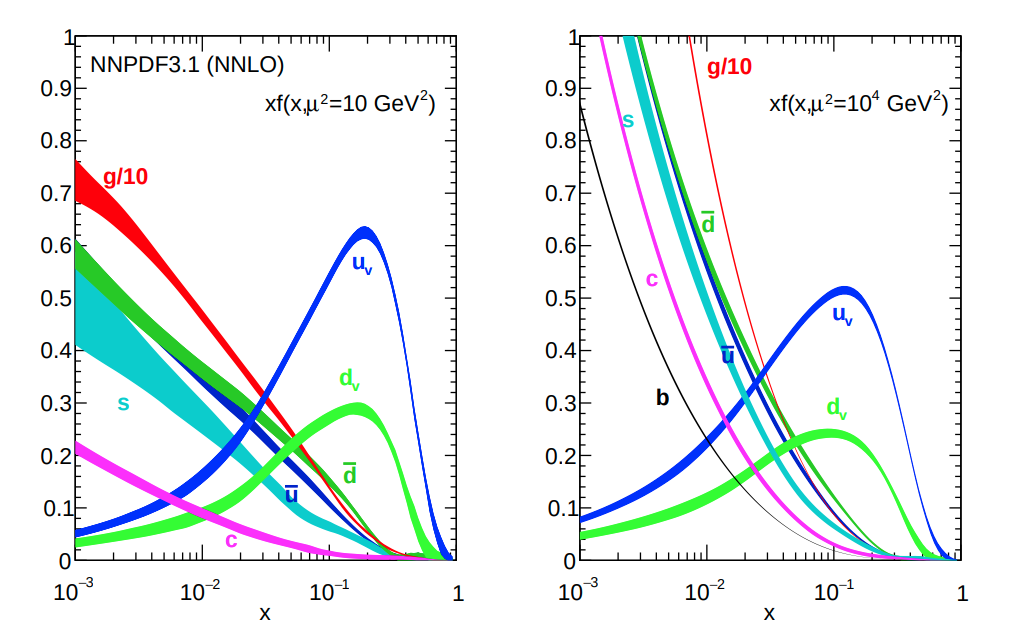
\includegraphics[width=12cm]{{img/NNPDF3.1.png}}
	\caption{The NNPDF3.1 NNLO PDFs set, evaluated at $Q^2 = 10\ \mathrm{GeV}^2$
(left) and $Q^2=10^4\ \mathrm{GeV}^2$ (right). At low $x$ the contribution from the gluons is the dominating one while at higher x the dominant contribution is from the valence quarks. The PDF $Q$ evolution shows that when our proton is probed to higher $Q^2$ the resolution increase (higher $Q$ correspond to smaller distance resolution) and so we have a bigger contribution from the sea quarks at low $x$ values.}
	\label{fig:NNPDF31}
\end{figure}
Note that the gluon contribution have been scaled of a factor 10: in fact, in the low $x$ region, $x<0.01$, the gluon contribution is the dominating one, while at high $x$ value the valence quarks dominate the PDF. 
\\
In \figRef{fig:NNPDF31} we can also see that with increasing virtuality ($Q^2$) at low $x$ the density of the sea quarks increases: this is related to the fact that our hadrons are probed at higher energy and the probe resolution is proportional to the energy. 
\begin{equation}
	\text{Resolution}\sim\frac{\hbar}{Q}\quad .
\end{equation}
So, when probed at higher energy, the hadrons appear denser\footnote{This density growth is not endless but at some point a saturation is reached it is called \textit{parton saturation}. The parton saturation find an explanation in the observation that at some high energy scale the parton mergers have to eventually compensate for splittings.} than when are probed at lower energy. This, as will be discussed in the below sections, is related to the energy dependence in the number of interaction between partons in a single hadron-hadron collision. The phenomenon of having more than one interaction between partons in a single hadron-hadron collision is called \textit{multiple parton interaction}: this concept will be discussed in the next chapter.

%%%%%%


%At this point the \emph{finite} corrections to the leading-logarithmic cross section in the perturbative expansion are specific for each process (i.e. they are not universal, but they are process dependent). This leads in the \eqRef{eq:factorization2} to the following series in $\alpha_s$ (the coupling constant of QCD theory):
%\begin{equation}
%	\sigma_{AB}=\displaystyle\int dx_a\,dx_b\,f_{a/A}(x_a,\mu_F^2)\,f_{b/B}(x_b,\mu_F^2)\,\left[\hat{\sigma}_0+\alpha_s(\mu_R^2)\hat{\sigma}_1+\dots\right]\quad .
%\label{eq:factorization3}
%\end{equation}
%In \eqRef{eq:factorization3} two scales enter the formula:
%\begin{itemize}
%	\item[--] The \textit{factorization scale} $\mu_F$: this scale is related to the resolution with which the hadron is being probed, separates long- and short- distance physics processes.
%	\item[--] The \textit{renormalization scale} $\mu_R$: the scale at which is evaluated the strong coupling constant $\alpha_s$. The dependence of $\alpha_s$ on the renormalization scale is related to different effects such as  the vacuum polarization, the quark self-energy, the vertex corrections, and the gluon loop corrections to the elementary three-gluon and four-gluon couplings.
%\end{itemize}
%
%The higher-order corrections to the cross section in \eqRef{eq:factorization3} are important because they lead to an higher accuracy in the cross section prediction, gradually reducing the dependencies on $\mu_R$ and $\mu_F$. In absence of an all-order prediction, a choice for the two scales have to be taken.
%Typically, the scales are assumed to be equal: in the Drell-Yan process the standard choice is $\mu_F=\mu_R=M$, with $M$ the lepton-pair mass \cite{Campbell2006}; other cases are the invariant masses of $Z$-boson, top quark or jet transverse energy to study \cite{Campbell2006} the production cross sections for Z-bosons, top quarks and large $E_T$ jets respectively.
%
%The parton distribution functions used to describe a hard scattering are solution to the DGLAP (Dokshitzer–Gribov–Lipatov–Altarelli–Parisi) equations \cite{Lipatov:400357, Gribov:427157, ALTARELLI1977298, Dokshitzer:1977sg}
%\\
%\begin{equation}
%	\mu_F^2\frac{\partial f_{i/H}(x,\mu_F^2)}{\partial\mu_F^2}=\displaystyle\sum_j\frac{\alpha_s(\mu_F^2)}{2\pi}\displaystyle\int_x^1 \frac{dz}{z}\, P_{i\,\rightarrow\,j}(z)\ f_{j/p}\left(\frac{x}{z},\mu_F^2\right)\quad ,
%\end{equation}
%\\
%where $P_{i\,\rightarrow\,j}$ are the so-called splitting functions: they are the probability that a parton of type $i$ emits a parton $j$ (a quark or a gluon) carrying a fraction $z$ of the $i$-parton momentum.
%\\
%The splitting functions have the following perturbative expansions in $alpha_s$: 
%\begin{equation}
%	P_{i\,\rightarrow\,j}(x,\alpha_s)=P_{i\,\rightarrow\,j}^{(0)}(x)+\frac{\alpha_s}{2\pi}P_{i\,\rightarrow\,j}^{(1)}(x)+\dots\quad .
%\end{equation}
%\\
%This procedure has been used to calculate cross-sections for many Standard Model processes in $p\overline{p}$ and $pp$ scattering respectively at Tevatron and LHC energies as shown in \figRef{figure:StandardModelCrossSections}.
%
%\begin{figure}[!htb]
%	\centering 
%	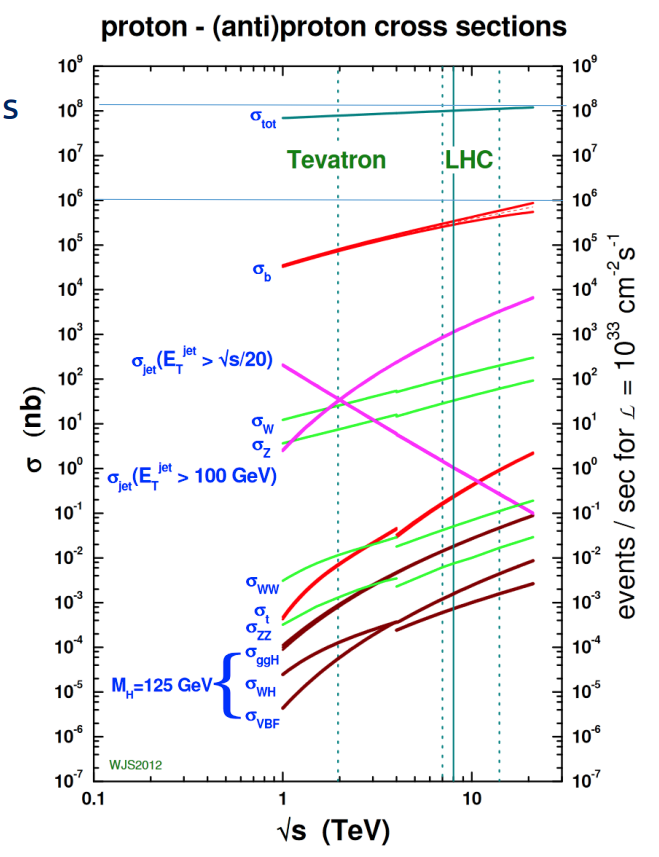
\includegraphics[width=12cm]{img/StandardModelCrossSections_color.png}
%	\caption{Next-to-leading order cross sections at Tevatron and LHC colliders energies (the splitting are at the transition between $p\overline{p}$ and $pp$ cross section). Figure from \cite{StirlingPrivate}}
%	\label{figure:StandardModelCrossSections}
%\end{figure}
%
%The parton distribution functions dependence on $Q^2$ can be derived theoretically via the DGLAP equations. Instead, the $x$ dependence is obtained fitting the deep-inelastic and other hard-scattering processes experimental data.
%The experimental coverage in $(x,Q^2)$-plane is shown in \figRef{figure:xQ2planeCoverage} 
%where is also underlined the relationship between $(x,Q^2)$ and kinematic variables in Drell-Yan processes for a final state with invariant mass $M$ and rapidity $y$ (further details in section 2 of \cite{Campbell2006}). Assuming that the factorization scale $Q$ is equal to $M$ (The reference center of mass energy is $13\ \mathrm{TeV}$), for two incoming partons with four-momentum respectively $p_1$ and $p_2$, the relations of their x (labeled as $x_1$ and $x_2$) with $s$, $y$ and $M$ are:  
%\begin{equation}
%	\begin{aligned}
%		&p_1^\mu=\frac{\sqrt{s}}{2}(x_1,0,0,x_1)\\
%&p_2^\mu=\frac{\sqrt{s}}{2}(x_2,0,0,-x_2)
%	\end{aligned} \quad\Longrightarrow\quad x_1=\frac{M}{\sqrt{s}}e^y\qquad x_2=\frac{M}{\sqrt{s}}e^{-y} \quad ,
%\end{equation}
%where  $s=(p_1^\mu+p_2^\mu)^2$. For example the figure shows that the production of a final state with invariant mass $M=100\ \mathrm{GeV}$ and rapidity $y=2$ is given by the interaction of two hadrons with $x_1\approx0.05$  and $x_2\approx0.001$ with $Q^2=10^4\ \mathrm{GeV^2}$
%
%
%\begin{figure}[!htb]
%	\centering 	
%	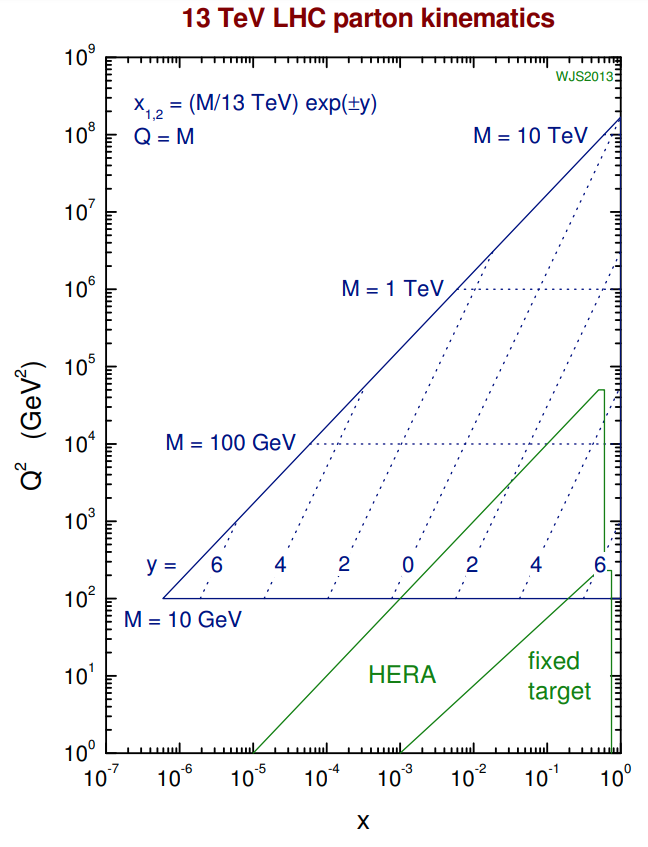
\includegraphics[width=12cm]{img/xQ2planeCoverage.png}
%	\caption{Graphical representation of the parton $(x,Q^2)$ variables coverage of different experiments. For LHC these $x$ and $Q^2$ are related to the kinematic variables $y$ and $M$. Figure from \cite{StirlingPrivate}}
%		\label{figure:xQ2planeCoverage}
%\end{figure}

\subsection{Partonic cross-section}

Partonic cross section is another fundamental ingredients in our recipe for the description of hadron-hadron interactions. It can be calculated as a perturbative expansion in $\alpha_s$ from QCD first principles using quantum field theory. So our hadron-hadron cross-section can be written as a sum of different contributions, as shown in the following formula:
\begin{equation}
	\sigma_{AB}=\displaystyle\int dx_a\,dx_b\,f_{a/A}(x_a,\mu_F^2)\,f_{b/B}(x_b,\mu_F^2)\,\left[\hat{\sigma}_0+\alpha_s(\mu_R^2)\hat{\sigma}_1+\dots\right]\quad .
\label{eq:factorization3}
\end{equation}
Where we have introduced the dependencies on the two unphysical scales:
\begin{itemize}
	\item[--] The \textit{factorization scale} $\mu_F$: this scale is related to the resolution with which the hadron is being probed, separates long- and short- distance physics processes.
	\item[--] The \textit{renormalization scale} $\mu_R$: the scale at which is evaluated the strong coupling constant $\alpha_s$. The dependence of $\alpha_s$ on the renormalization scale is related to different effects such as  the vacuum polarization, the quark self-energy, the vertex corrections, and the gluon loop corrections to the elementary three-gluon and four-gluon couplings.
\end{itemize}
The calculation of such expansion at the leading order (LO) is performed by evaluating all the possible tree-level Feynman diagrams for every process. Then the calculation proceeds by computing the squared matrix element and by integrating it over the available phase space (analytically or numerically).
\\
At this point, we can already encounter some divergence that can be avoided imposing some  restrictions on the phase space.
% restriction or constraints

\subsubsection{Higher order calculations}

The LO calculation can describe broad feature of a particular process and provide a first estimation of its cross section; anyway, in many cases this is insufficient.
\\
The main source of uncertainty derives from the LO dependence  on the unphysical renormalization and factorization scales. Some process may contribute only when going beyond the first approximation, and some divergence can be resummed. 
\\
The next-to-leading order (NLO) calculation requires all the Feynman diagrams that take an extra $\alpha_s$. This contribution can arise in two different ways:
\begin{itemize}
	\item \textbf{Virtual}: internal lines in the Feynamn diagram, see \figRef{fig:feynman_Real_Virtual}a, that don't originate a real particle in the initial or in the final state (loops);
	\item \textbf{Real}: external lines int the Feynamn diagram, see \figRef{fig:feynman_Real_Virtual}b, here the particle is real and participate to the initial or final state observed (real particles).
\end{itemize}
\begin{figure}[!htb]
	\centering
	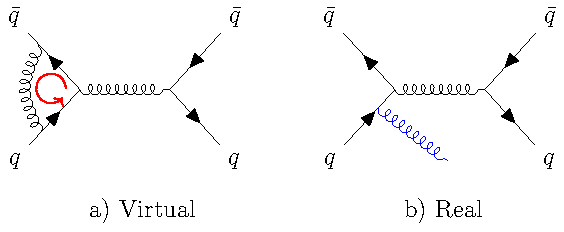
\includegraphics[width=0.7\textwidth]{img/feynman_Real_Virtual.pdf}
	\caption{Feynamn diagrams for a virtual correction (a) the momentum circulating in the loop when integrated on the phase space take to a divergence; and a real correction (b) the particle emitted is real, participate to the initial or final state of the process.}
	\label{fig:feynman_Real_Virtual}
\end{figure}

Virtual corrections contains infrared divergences, arising by integrating on the loop circulating momentum, that cancel against infrared singularities given by collinear  or soft emissions \cite{PhysRevBloch, KinoshitaToichiro, PhysRevLee}. 
\\
A common strategy for the renormalization is dimensional regularization: it consists into performing the calculation in a $D=4-2\epsilon$ dimensional space ($\epsilon<0$); in that way the singularities appear as single and double poles in $\epsilon$. Then, the limit $\epsilon\rightarrow0$ is taken after the divergences have cancelled.
\\
This NLO calculation with regularization allows to extend the treatment of these integrals up to zero transverse momentum.

The importance of higher-order calculation is that it allows too describe more processes, as can be shown with the following example. In a $Z$ boson production:
\begin{enumerate}[label=$\arabic*)$]
	\item \textbf{LO}: the $Z$ is produced without transverse momentum ($p_T$), and anything can recoil against the $Z$ for momentum conservation (\figRef{fig:Zprod_feynman_LO_NLO_NNLO}{\color{blue}{a}}). 
	\item \textbf{NLO}: the $Z$ acquires a finite $p_T$. In this case the $Z$ boson $p_T$ is balanced by a single \mbox{parton/gluon} (\figRef{fig:Zprod_feynman_LO_NLO_NNLO}{\color{blue}{b}}).
	\item  \textbf{NNLO}: the $Z$ $p_T$ can be balanced by two jets (\figRef{fig:Zprod_feynman_LO_NLO_NNLO}{\color{blue}{c}}). 
\end{enumerate}
\begin{figure}[!htb]
 \centering
 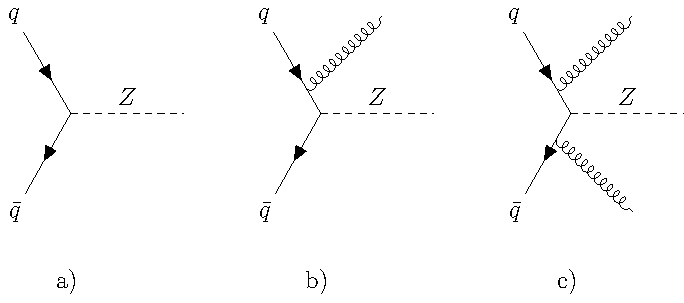
\includegraphics[width=12cm]{{img/feynman_ZpT.pdf}}
 \caption{Feynman diagrams for the Z production by annihilation of a quark and an antiquark at LO (a), NLO (b), NNLO (c). At LO the $Z$ can only be produced with a $p_T=0$ for the conservation of the momentum.}
 \label{fig:Zprod_feynman_LO_NLO_NNLO}
\end{figure}
Another important benefit of performing a NLO calculation is the the reduction of the dependence of calculation on the unphysical renormalization ($\mu_R$) and factorization ($\mu_F$) scales.
It is proven that higher order calculations of observables calculated to order $\alpha_s^{\,n}$ are dependent upon the unphysical scales only at order higher than $\alpha_s^{\,n+1}$ \cite{Campbell2006}. The range of predictions corresponding to different scale choices is usually attributed to \textit{theoretical uncertainties}, as is shown in \figRef{fig:ZRapidityDistributionLO_NLO_NNLO}, where the uncertainties reduce from the LO calculation to the NLO and even more to the NNLO.

\begin{figure}[!htb]
	\centering
	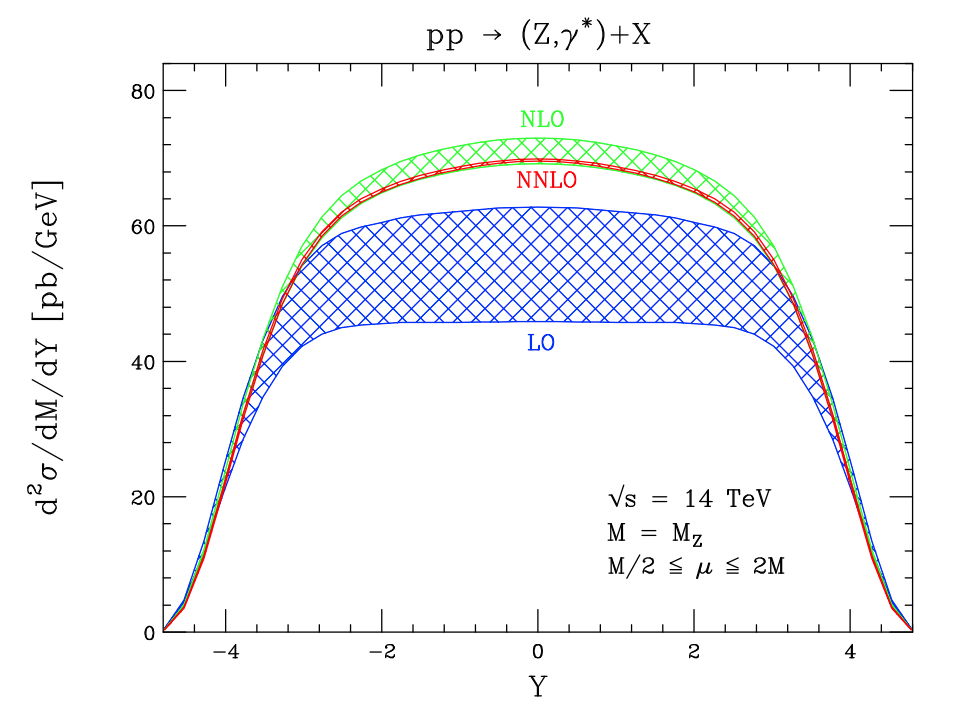
\includegraphics[width=12cm]{{img/ZRapidityDistributionLO_NLO_NNLO.png}}
	\caption{The rapidity distribution predictions at LO (blue) NLO (green) and NNLO (red) for the Z production at the center of mass energy$\sqrt{s}=14\ \mathrm{TeV}$. The band width is related to the uncertainties. Going from LO to NLO there is a increase in the cross section prediction and a reduction on the scales uncertainties, the NNLO prediction is in the NLO error band width but there is a further increase in the precision of the prediction. Figure from \cite{Campbell2006}, section 6.}
	\label{fig:ZRapidityDistributionLO_NLO_NNLO}
\end{figure}

%\section{Parton Showers}
%
%A different approach to describe the phenomena observed at high-energy colliders, instead of calculating cross sections order by order in the perturbative expansion, is the use of an \textit{all-order} approach. 
%\\
%Different all-order approaches exist such as resummation techniques and parton showers. Resummation is based on the observation that in many quantities the smallness of the expansion coefficients $\alpha_s$ is violated by large logarithmic enhancements. This takes the dominant contribution from each order and "resums" them by means of an evolution equation. 
%The main problem in QCD is related to the fact that lot of quantities have corrections of the form $\alpha_s^n\log^k(Q_i/Q_j)$ where $Q_i$ and $Q_j$ are two different energies scales, for example:
%\begin{itemize}
%	\item[--] Renormalization $\mu_R=Q^2$ and factorization scales logs: $\alpha_s^n\log^n(Q^2/\mu_f)$
%\end{itemize}
%Various methods to perform this resummation exist.
%\\
%%%%% GRAPH on pT Z with effect of resummation 
%An example is the $Z$ production $p_T$ spectrum shown in \figRef{figure:pT_Z_CDF}: here the comparison between experimental CDF data and theoretical predictions is shown: in the low $p_T$ region the \textit{all-order} approach regularizes the divergence of the fixed order calculation and describes the data better. 
%
%\begin{figure}[!htb]
%	\centering
%	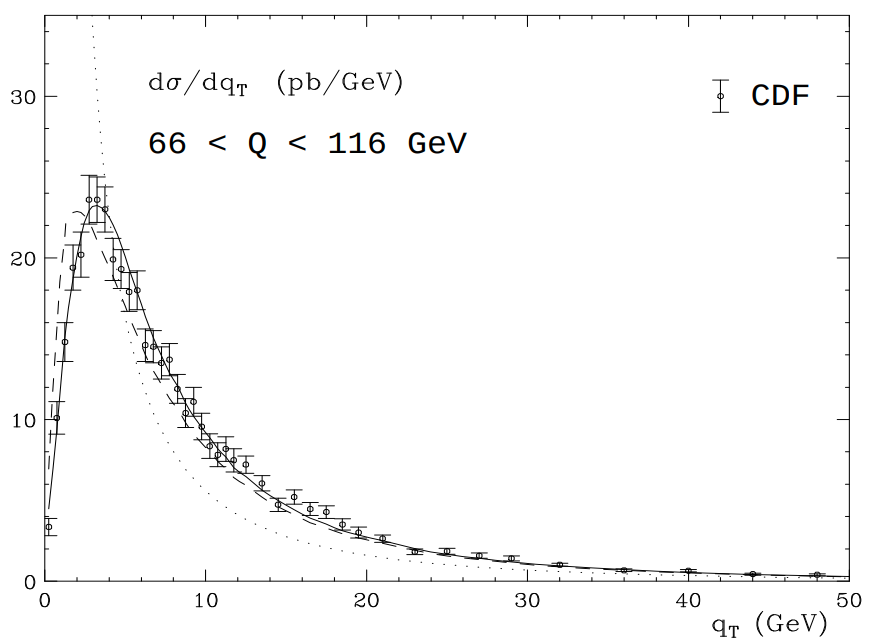
\includegraphics[width=12cm]{{img/pT_Z_CDF.png}}
%	\caption{CDF data on $Z$ production cross section at Tevatron collider, CDF experiment, the predictions from fixed order calculation (dotted) with resummation (dashed), and with the inclusion of power corrections (solid) are compared. Figure take from \cite{kulesza2002electroweak}}
%	\label{figure:pT_Z_CDF}
%\end{figure}
%
%An other \textit{all-order} approach is based on the simulation of the so-called "parton showers". It is  implemented in different Monte Carlo programs, as  \textsc{pythia} \cite{PYTHIA2015}, \textsc{herwig} \cite{Herwig2008} and \textsc{sherpa} \cite{SHERPA2004}. 
%The algorithm starts from few partons arising from a hard interaction. Then, as the energy scale at which we examines the scattering decrease these harder partons can split, and so more partons are produced in the shower. The higher scale parton are related to the lower energy scale (close to $\Lambda_{QCD}$) using the DGLAP evolution equation formalism. The solution to this equation can be written using a Sudakov form factor arising from the probability of no gluon emission in the evolution from higher to lower scale.
%\\
%In the parton showering process, in addition to the kinematic variables (momentum fraction $z$ and azimuthal angle $\phi$) and flavours of the partons, an evolution variable $t$ is generated. \textsc{Pythia8} uses as  evolution variable the squared of the relative transverse momentum of the two partons in the splitting ($p_T^2$). Different choices are made in \textsc{herwig} and \textsc{sherpa}.
%\\
%As mentioned before, the shower evolution is based on the standard (LO) DGLAP splitting kernels P(z) described here:
%\begin{align}
%P_{q\,\rightarrow\,qg}(z) & = C_F\frac{1+z^2}{1-z}\quad ; \\
%P_{g\,\rightarrow\,gg}(z) & = C_A\frac{(1-z(1-z))^2}{z(1-z)}\quad ; \\
%P_{q\,\rightarrow\,q\overline{q}}(z) & = T_R(z^2+(1-z)^2)\quad ;
%\end{align} 
%where $C_F=\frac{4}{3}$ is the Casimir operator for $SU(3)$, $C_A=N_C=3$, that are named "color factors", and $T_R=\frac{1}{2}$ that is given by the trace calculation of the group generators, each contribution is multiplied by $N_f$ if summing over all contributing quark flavours.
%\\
%The parton shower consist of two components: the initial-state radiation (ISR) describing the emission from the incoming partons and the final-state radiation (FSR) describing emission of outgoing partons.
%Both ISR and FSR algorithms are based on these splitting kernels.
%The respective probabilities of emitting radiation as one moves in the decreasing evolution variable sequence are:
%\begin{align}
%	FSR: \qquad\quad & \frac{d\mathcal{P}_{FSR}}{dp_T^2} = \frac{1}{p_T^2}\displaystyle\int \frac{dz}{z}\,\frac{\alpha_s}{2\pi}P(z)\quad ;\label{eq:FSR1}\\
%	ISR: \qquad\quad & \frac{d\mathcal{P}_{ISR}}{dp_T^2} = \frac{1}{p_T^2}\displaystyle\int \frac{dz}{z}\,\frac{\alpha_s}{2\pi}P(z)\,\frac{f'(x/z,p_T^2)}{f(x,p_T^2)}\quad .\label{eq:ISR1}
%\end{align}
%We can write-out our Sudakov form factor by using the two probability in \eqRef{eq:FSR1} and \eqRef{eq:ISR1}, as
%\begin{equation}
%	\Delta(p_T^2)=\exp\left( -\displaystyle\int_{p_T0}^{p_T'} \frac{d\mathcal{P}_{PS}}{dp_T^2} \,dp_T\right) \qquad\text{ with } \quad PS=ISR,\ FSR \quad.
%	\label{eq:sudakovFormFactor}
%\end{equation}
%The Sudakov form factor give the probability of a parton to evolve from an harder scale to a softer scale without emitting a parton harder than some resolution scale. 
%\\
%The introduction of the Sudakov form factor resums all the effects from the soft and collinear gluon emission. For more details and some plots of different Sudakov form factor values see section 3.5 of \cite{Campbell2006}.
%
%\subsection{Merging parton showers and matrix element calculations}
%
%Regions dominated by soft and collinear gluon emissions are described very well by parton showers approach; on the other hand, regions where partons are  energetic and widely separated are well described by matrix element calculations.  
%So, the best approach would be to combine the two different descriptions, this would require an universal formalism for parton showers and matrix element calculations. This universal formalism was created in 2001 and it is called "Les Houches Accord" \cite{LesHouchesAccord}.
%In order to combine the two approaches some care must be taken: there is the risk of double counting. Different techniques prevent this risk: for example CKKW \cite{CKKW2001} is used to combine LO matrix element calculations and parton shower.
%
%
%A better way is to combine NLO matrix element calculation with parton showers: this is done by the FxFx mergin scheme, developed by Frixione, Nason, Webber in the \textsc{mc@nlo} framework \cite{FxFx1,FxFx2,FxFx3,FxFx4}. In this scenario the risk of  double counting is given by the fact that at NLO one emission can be made explicit as indicated in \figRef{fig:DoubleCounting} by the red gluon line, then the progress of the parton shower can leads to a double counting between real emission matrix element and the parton shower as shown in \figRef{fig:DoubleCounting}, the double counting sources are indicated by the blue arrows.
%% TODO: mi piacerebbe aggiungere una descrizione più completa del merging con FxFx visto che viene usato dopo. 
%
%%%%
%%%% Immagine di Frixi.. presentation
%\begin{figure}[H]
%	\centering
%	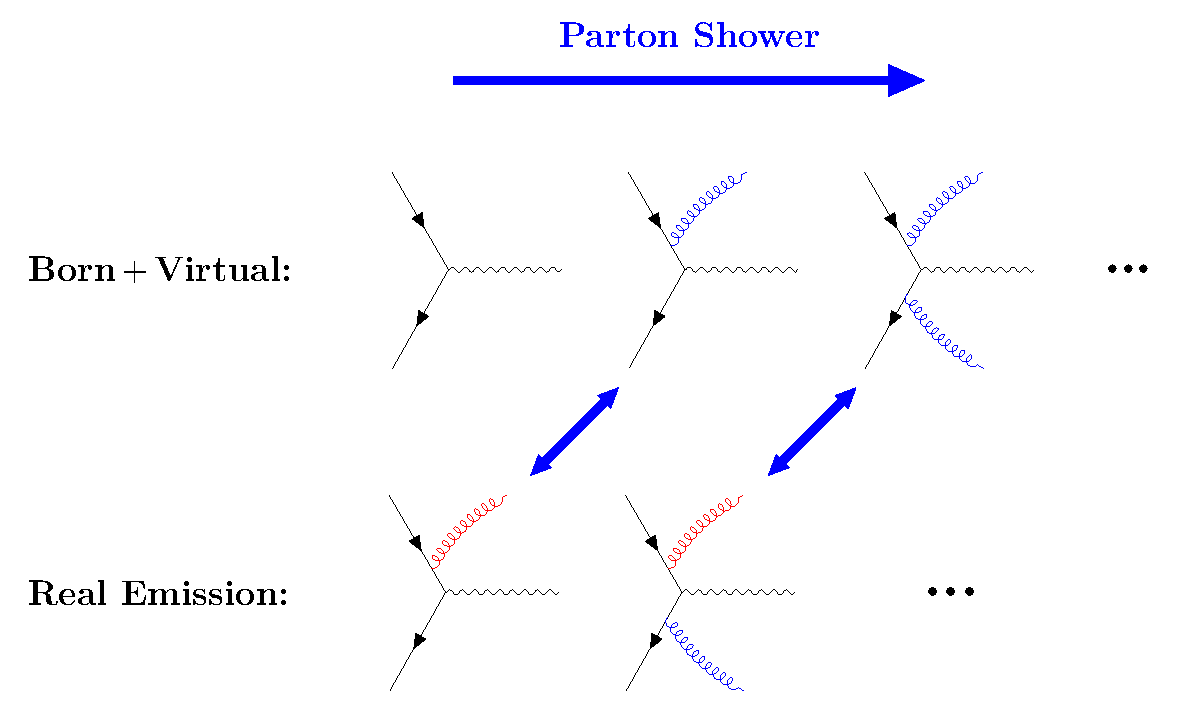
\includegraphics[width=14cm]{{img/feynman_doubleCounting_FxFx_curved-cropped.pdf}}
%	%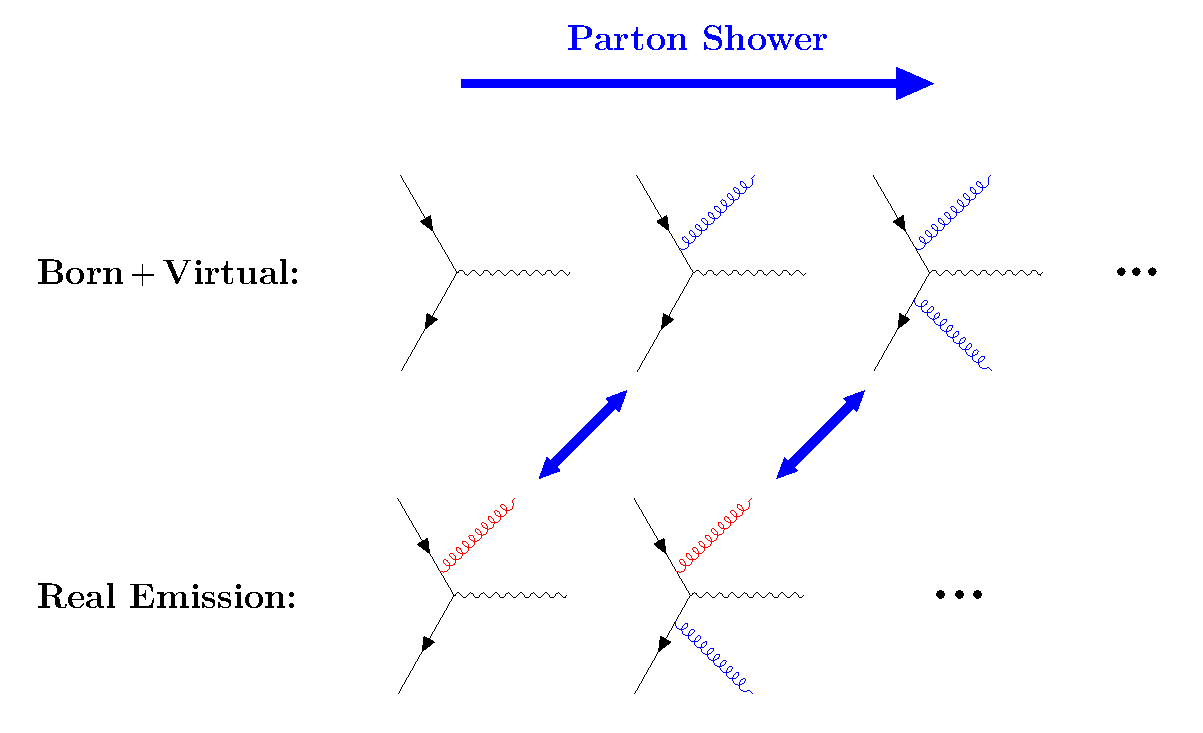
\includegraphics[width=14cm]{{img/feynman_doubleCounting_FxFx-cropped.pdf}}
%	\caption{The FxFx margin scheme have to avoid this double counting. Feynman diagrams that can lead to a double counting are grouped with the violet arrow, the blue emission are related to the parton shower while the red ones to the NLO process.}
%	\label{fig:DoubleCounting}
%\end{figure}
%%%%


%\section{Parton distribution functions}
%
%The last ingredient in our recipe is the knowledge of the quark and gluon distributions inside the two hadrons that undergo the scattering. We have already seen that these quantities are depending on the virtuality ($Q^2$) of the interaction.
%\\
%The information on the quark distribution inside a hadron $f_{q/p}(x,Q^2)$ arises from lepton-hadron DIS experiments, from lepton-pair production in hadron-hadron collisions (Drell-Yan processes) and jet measurements to study gluon distribution $f_{g/p}(x,Q^2)$. All these quantities are the experimental input in order to evaluate the PDF inside the hadron while the $Q$-evolution is described by DGLAP equation.
%The evolution of the PDF can be run either with a NLO or with a NNLO calculations.
%
%The kinematic region covered by experiments is shown in \figRef{figure:xQ2planeCoverage}. At very low x and $Q^2$ the DGLAP evolution is believed to be no longer applicable and a BFKL (Balitsky-Fadin-Kuraev-Lipatov) \cite{BFKL1,BFKL2} description must be used.
%%;
%%anyway, this has not any experimental evidence so the DGLAP approach is used as default in all the PDF analysis.
%% but there are no experimental evidence of this so the DGLAP approach is used as default in all the PDF analysis.
%\\
%A lot of processes are available for the PDFs evaluation and a lot of PDF set have been generated, as an example \figRef{fig:NNPDF31} shows the NNPDF3.1 set \cite{NNPDF3.1} at NNLO for a virtuality $Q^2=10\ \mathrm{GeV^2}$ (left) and $Q^2=10^4\ \mathrm{GeV^2}$ (right). 
%\begin{figure}[!htb]
%	\centering
%	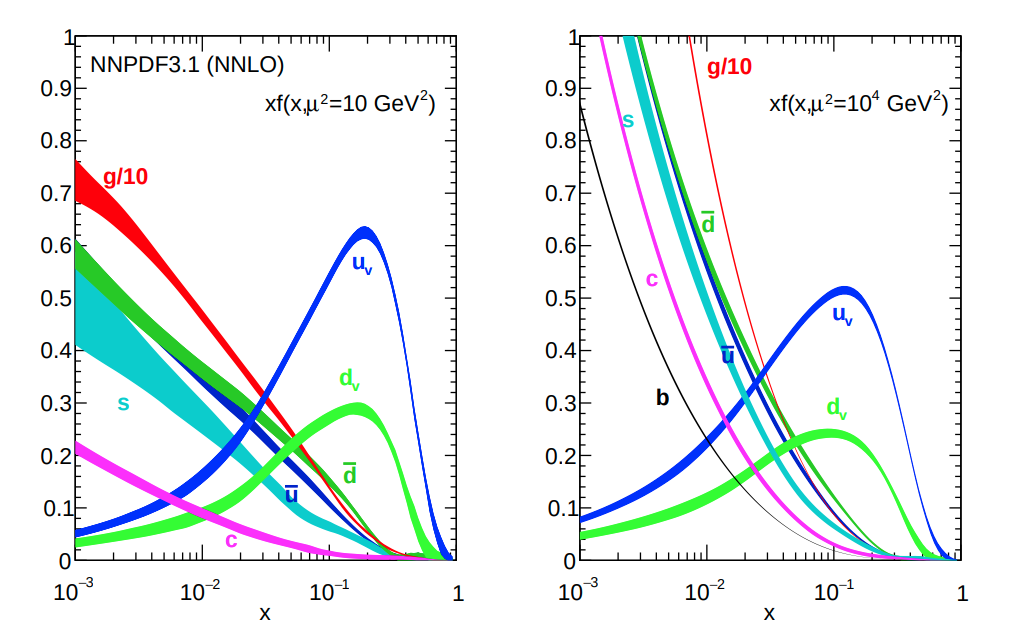
\includegraphics[width=12cm]{{img/NNPDF3.1.png}}
%	\caption{The NNPDF3.1 NNLO PDFs set, evaluated at $Q^2 = 10\ \mathrm{GeV}^2$
%(left) and $Q^2=10^4\ \mathrm{GeV}^2$ (right). At low $x$ the contribution from the gluons is the dominating one while at higher x the dominant contribution is from the valence quarks. The PDF $Q$ evolution shows that when our proton is probed to higher $Q^2$ the resolution increase (higher $Q$ correspond to smaller distance resolution) and so we have a bigger contribution from the sea quarks at low $x$ values.}
%	\label{fig:NNPDF31}
%\end{figure}
%Note that the gluon contribution have been scaled of a factor 10: in fact, in the low $x$ region, $x<0.01$, the gluon contribution is the dominating one, while at high $x$ value the valence quarks dominate the PDF. 
%\\
%In \figRef{fig:NNPDF31} we can also see that with increasing virtuality ($Q^2$) at low $x$ the density of the sea quarks increases: this is related to the fact that our hadrons are probed at higher energy and the probe resolution is proportional to the energy. 
%\begin{equation}
%	\text{Resolution}\sim\frac{\hbar}{Q}\quad .
%\end{equation}
%So, when probed at higher energy, the hadrons appear denser\footnote{This density growth is not endless but at some point a saturation is reached it is called \textit{parton saturation}. The parton saturation find an explanation in the observation that at some high energy scale the parton mergers have to eventually compensate for splittings.} than when are probed at lower energy. This, as will be discussed in the next chapter, is related to the higher number of interaction between partons in a single hadron-hadron collision. The phenomenon of having more than one interaction between partons in a single hadron-hadron collision is called \textit{multiple parton interaction}: this concept will be discussed in the next chapter.

%
%\section{A real proton-proton collision}
%
%
%We have understood that the complexity in the description of a proton-proton collision arises from composite nature of the protons. In this chapter we discussed the importance of the QCD factorization theorem that help us in the calculation of the hadronic cross section with the convolution between the partonic cross section and the parton distribution functions (PDF). We have discussed the importance of the parton shower algorithm where a set of partons are evolved in a more complex final state by emissions in the initial and final states.
%\\
%All these processes are important in the description of a real proton-proton collision but also the partons that are left unscattered are non-color singlet and can contribute to the complex final state observed in the experiments, and additionally, as mentioned before, nothing prevent additional partons scatterings from taking place and increasing more and more the complexity of the partons final state. 
%
%Another problem is related to the not-well-understood hadronization process of all the final-state partons involved in the hadron-hadron interaction.
%Hadronization is not known from first principles and different models have been implemented in different programs: the \textit{cluster fragmentation model} implemented in \textsc{herwig} and the \textit{string fragmentation model} in \textsc{pythia}
%%simulated this process of hadronization where the set of final-state partons is transformed into a set of hadrons. 
%All these processes are schematically shown in \figRef{fig:Processes}.
%
%\begin{figure}[!htb]
%	\centering
%	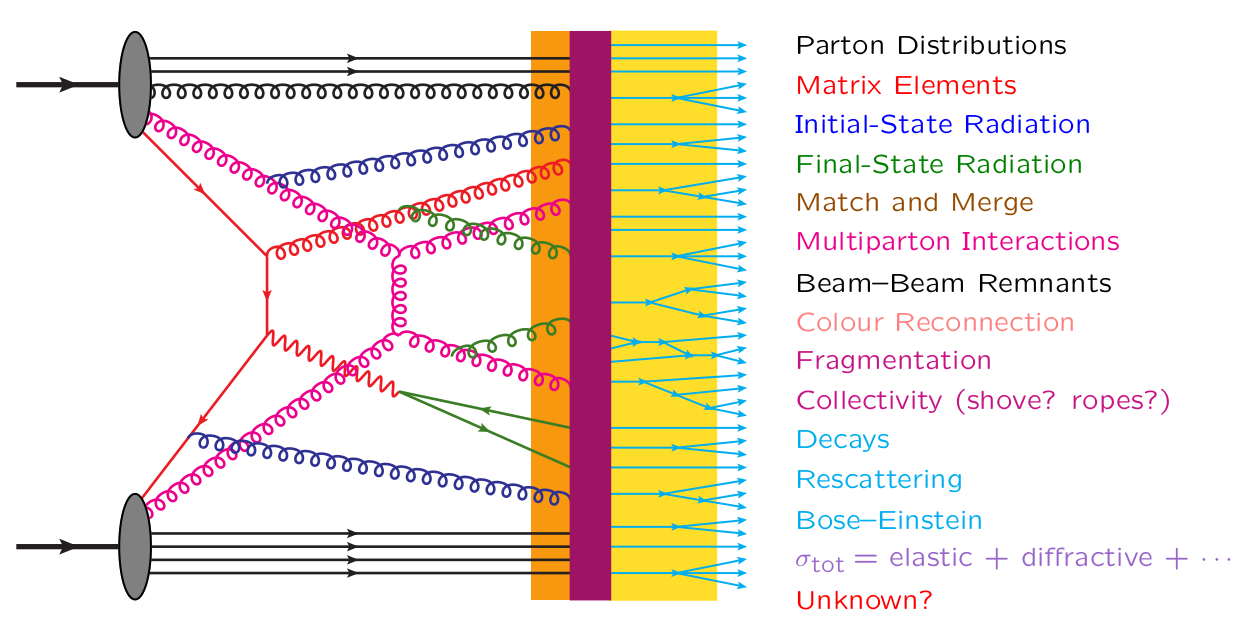
\includegraphics[width=0.98\textwidth]{{img/Processes.png}}
%	\caption{A schematic representation for a $pp$ collision. Reading the image from left to right one can have an idea on the evolution of the system. The two incoming hadrons enter the scattering from the left side, the red line indicate the main hard scattering and the magenta one the second parton scattering (MPI) each interaction is associated with initial (blue) and final (green) state radiation, the unscattered partons (black lines) re-enter the color reconnection and hadronization processes. Than the new formed hadrons (lightblue) can undergo to different decays.}
%	\label{fig:Processes}
%\end{figure}
%
%Next chapter will describe in more details  the \textsc{pythia} Monte Carlo generator, that is currently used to simulate many processes in proton-proton collision at the LHC. \textsc{pythia} introduces different free parameters that need to be tuned with experimental data (from Tevatron and LHC). The tune methods are described in \chapRef{chap:TuneprocedureCP5TuneandMCNNTUNES} along with the description of some already existing tune for the underlying event in proton-proton collision.



%%% ---



%In a \textbf{proton-proton collision}, additionally to the main hard scattering that can be described performing Matrix Element calculations (MEs) , also other scattering processes are possible. To well understood the proton-proton collision we need to describe other processes, besides to the hard scattering, that can underlying to this  \textbf{Multi Parton Interaction} (MPI) and the \textbf{Beam-Beam Remnants} (BBR).




%\end{document}